% Example on how to use the QPSR LaTeX2e class
\documentclass[a4paper,twoside,10pt]{fonetik}

% These are optional packages if you like:
% - nice fonts and symbols for mathematics
\usepackage{amsmath,amsfonts,latexsym,amssymb}
% - input and font encoding for european languages (accented
%   letters). If not used, you need to type Swedish letters,
%   for example with LaTeX commands: \"a \"o \aa \"A \"O \AA
\usepackage[latin1]{inputenc}
\usepackage[T1]{fontenc}
% - language specific definitions (if not English)
%\usepackage[english]{babel}
% - extends the tabular syntax for tables.
\usepackage{array}
% - to insert nice eps figures
\usepackage{graphicx}

% defining hyphenation for difficult words is also optional
\hyphenation{si-mu-la-tion re-so-nance mo-dels}

% here you can also define some commands that you want to use
% later to simplify typing text
\newcommand{\BibTeX}{{\rm B\kern-.05em{\sc i\kern-.025em b}\kern-.08em
    T\kern-.1667em\lower.7ex\hbox{E}\kern-.125emX}}

% These are definitions used to create the header and footer.
% Ask the values for first page, volume and publication year
% to Cathrin
\volume{45}
\pubyear{2004}
\firstpage{69}

% Here is the title, author and abstract definition
% Note:
% 1) affiliation should not specified if it is TMH
% 2) the abstract is defined in a nonstandard way
\title{An example on using the QPSR \LaTeX2e class}
\author{Giampiero Salvi}
\affiliation{Here write the affiliation only if it is different from TMH}
\abstracttext{This is an example on how to use the \LaTeX2e class {\tt
  qpsr.cls} for writing articles in the style adopted by the Quartely
Progress and Status Report (QPSR) at the department for Speech, Music
and Hearing (TMH) at the Royal Institute of Technology (KTH) in
Stockholm. This example will describe some of the standard features of
\LaTeX2e and the additional commands provided by the class.}

\begin{document}
\maketitle

% This is probably optional, depending on what characters you
% want to type.
%\fontencoding{OT1}

% note that defining labels for sections is useless, as there is no
% numbering in the QPSR style (unfortunately).
\section{Introduction}
Provided that you have the \verb|qpsr.cls| file in the same directory
as the \verb|.tex| file, or somewhere in the \LaTeX\ search path, the
document class is specified by the command:
\begin{verbatim}
\documentclass[a4paper,
       twoside,11pt]{qpsr}
\end{verbatim}

A number of packages can then be included depending of the special
needs of the author. This is done with the \verb|\usepackage| command
(look at the \verb|.tex| file in the distribution for examples).

The number of the first page is specified for example with the command
\verb|\firstpage{69}|. The volume number and the publication
year are specified by the commands (defined by the class)
\verb|\volume| and \verb|\pubyear|. These will appear, together with
the author's name and the title in the headers and footers for each
page. You should ask Cathrin Dunger for the right numbers to use. 

Title and author are defined as usual by the \verb|\title| and
\verb|\author| commands. A new command \verb|\affiliation| is provided
for affiliation. Note that this should be omitted if the affiliation
is the department for Speech, Music and Hearing. Another special
command is the \verb|\abstracttext|. Usually in \LaTeX\ the abstract
is defined using the environment \verb|abstract| after the
\verb|\begin{document}|
command. For technical reasons, here the
\verb|abstract| environment is not used, but rather the command
\verb|\abstracttext| is used in the preamble and the abstract is
generated by the \verb|\maketitle| command.

Sections, subsections\ldots, are started with the usual
\verb|\section|, \verb|\subsection|\ldots\ commands. There is no need
to use the ``starred'' version of these commands as numbering is
omitted by default.

For the rest, normal \LaTeX\ commands can be used to produce cross
references (\verb|\label| and \verb|\ref|), tables and figures, with
the corresponding environments, mathematical formulas, citations
(using the \verb|natbib| package that is automatically loaded by the
class). Note that setting labels to sections and subsections is
useless as there is no numbering in the QPSR style
(unfortunately). Examples of this and more can be found in the rest of
this document. In case you are reading a PostScript or PDF version of it
you are referred to the \verb|example.tex| file that was used to
generate them.

One of the best ways to produce a bibliography is to create a \BibTeX\
file (see \verb|example.bib| in the distribution). The citations can be
obtained by using one of the following commands. If the citation comes
in the end of a phrase, the \verb|\citep| command should be used,
e.g.
\begin{quote}
\ldots{}the first attempts to simulate the flow-induced oscillations
were based on a lumped- element model \citep{SmartAndSmarter68}.
\end{quote}
 If the author is cited directly in the text,
then the \verb|\citet| command should be used instead, e.g.
\begin{quote}
An essential improvement to the one-mass model was proposed by
\citet{DullAndMean98}, with their two-mass model.
\end{quote}
For more information, refer to the \BibTeX\ and {\tt natbib}
documentation \citep[e.g.][ch. 13]{companion}. Another good reference for
\LaTeX\ in general is \citep{short} (just google on the net).

\section{Inserting Figures and Tables}
Also the figures and tables can be inserted with standard \LaTeX\ 
commands. This is an example:
\begin{verbatim}
\begin{figure}
\centering
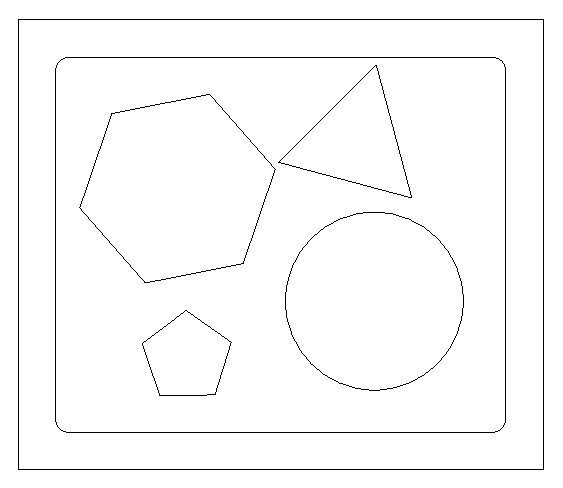
\includegraphics[scale=0.8]
  {figures/figb.eps}
\caption{An abstract figure.}
\label{fig:abstract}
\end{figure}
\end{verbatim}
The above code is used to produce Figure~\ref{fig:abstract}. Note that
I used the command \verb|\ref{fig:abstract}| to generate the figure
number in the previous sentence.
\begin{figure}
\center
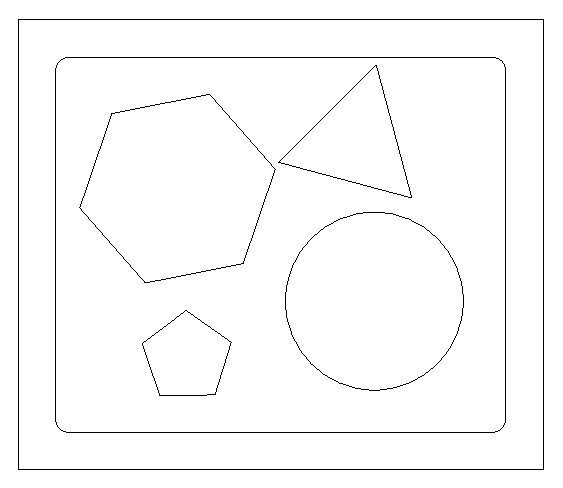
\includegraphics[scale=0.8]{figures/figb.eps}
\caption{An abstract figure.}\label{fig:abstract}
\end{figure}

If you want to include figures that span two columns, use the
``starred'' version of the {\tt figure} environment, i.e.
\begin{verbatim}
\begin{figure*}
...
\end{figure*}
\end{verbatim}
An example will be given later.

Inserting tables is as easy, just remember to put the caption above the
table, i.e
\begin{verbatim}
\begin{table}[b]
\centering
\caption{This is the table
   caption (above the table)}
\label{tab:example}
\begin{tabular}{cc}
  \hline \hline
  Parameter & Value \\
  \hline
  \\
  $m$ & $0.00017$ $kg$   \\
  $L$ & $0.014$ $m$ \\
  $x_0$ & $0.005-0.1$ $mm$ \\
  \hline \hline
\end{tabular}
\end{table}
\end{verbatim}

\begin{table}[b]
\centering
\caption{This is the table caption
  (above the table)}
\label{tab:example}
\begin{tabular}{cc}
  \hline \hline
     Parameter & Value \\
     \hline
     \\
      $m$ & $0.00017$ $kg$   \\
      $L$ & $0.014$ $m$ \\
      $x_0$ & $0.005-0.1$ $mm$ \\
      \hline \hline
\end{tabular}
\end{table}

The above code is used to generate Table~\ref{tab:example}. Note that in this
case I added the option {\tt [b]} that indicates I wish the table to
be at the bottom of the page, if possible. Other options for floating
object placement are: {\tt [h]} for ``here'', i.e. the insertion point
in the text, {\tt [t]} for ``top'' that is the default, and {\tt [p]}
to put it in a special page that collects all floating objects. These
options are just an indication of preference, and they are overridden
by other type-setting rules. If you want to strengthen your
determination against the evil computerised type-setter, put an
exclamation mark in front of the option (\verb|[!h]|), but note that
the type-setter is still setting the rules, to some extent.

\subsection{Lots of meaningful words}
This section is just a filler to come to the next page.

\begin{figure*}[!t]
\centering

\includegraphics[scale=0.6]{figures/figa.eps}
\caption{A more concrete figure.} \label{fig:concrete}
\end{figure*}
Peace and love peace and love peace and love peace and love peace and
love peace and love peace and love peace and love peace and love peace
and love peace and love peace and love peace and love peace and love

Peace and love peace and love peace and love peace and love peace and
love peace and love peace and love peace and love peace and love peace
and love peace and love peace and love peace and love peace and love

Peace and love peace and love peace and love peace and love peace and
love peace and love peace and love peace and love peace and love peace
and love peace and love peace and love peace and love peace and love

\subsection{It's never enough!}
Peace and love peace and love peace and love peace and love peace and
love peace and love peace and love peace and love peace and love peace
and love peace and love peace and love peace and love peace and love

Peace and love peace and love peace and love peace and love peace and
love peace and love peace and love peace and love peace and love peace
and love peace and love peace and love peace and love peace and love

Peace and love peace and love peace and love peace and love peace and
love peace and love peace and love peace and love peace and love peace
and love peace and love peace and love peace and love peace and love.

\section{A last example}
As promised in a previous section an example of a
two-column figure is Figure~\ref{fig:concrete}

\section{Last page and column balancing}
To balance the length of the two (incomplete) columns on the last
page, use the \verb|\balance| command. This sould be is issued before
the first column of the last page is finished. NOTE: this command can
cause problems with the displacement of floating objects (figures and
tables). If you encounter such problems, remove the command (you will
get unbalanced columns on the last page).
\balance


\section{Acknowledgement}
The author is grateful to all the nice people using \LaTeX\ to typeset
their contribution to the QPSR. This work has been supported by lots
of patience and a whole load of irresponsibility.


\bibliographystyle{qpsr}
\bibliography{example}

\end{document}
